\documentclass[12pt, letterpaper]{article}

\setlength{\topmargin}{-1.75cm} \setlength{\textheight}{22.5cm}
\setlength{\oddsidemargin}{0.25cm}
\setlength{\evensidemargin}{0.25cm} \setlength{\textwidth}{16.2cm}

% symbols 
\usepackage{fdsymbol}
\usepackage{stmaryrd}
\usepackage{pifont} % check/cross marks 
\newcommand{\cmark}{\ding{51}}%
\newcommand{\xmark}{\ding{55}}%
%\usepackage{amssymb}
\usepackage[ruled,linesnumbered]{algorithm2e}
\usepackage{graphicx}
\usepackage[linguistics]{forest}
% for automata 
\usepackage{tikz} 
\usetikzlibrary{automata,positioning}


\usepackage{palatino, url, multicol} % for multiple columns

\usepackage{pictex}
%% in the .pictex output of xfig, there is command \colo
%% however the old version of pictex may not define this
%% so we define color here as empty
\def \color#1]#2{}

\usepackage{fancyhdr}
\pagestyle{fancy}

\newcommand{\hwnumber} {
    6
}

\newcommand{\hwtitle} {
Turing Machine. Complexity.   
}

\newcommand{\duedate}{
    11:59 pm Sunday, November 28th}

\date{}

\begin{document}

\newcommand{\hide}[1]{}
\newcommand{\otherquestions}[1]{}
\newcommand{\set}[1]{\{#1\}}
\newcommand{\pg}[1]{{\tt #1}}
\newtheorem{definition}{Definition}
\newcommand{\emptyclause}{\Box}
\newcommand{\keyword}[1]{{\bf #1}}

\newcommand{\ee}[1] {
  \begin{enumerate}
    #1
  \end{enumerate}
}
%% \noindent test \hfill test

\newcommand{\ie}[1] {
  \begin{enumerate}
    #1
  \end{enumerate}
}

\newcommand{\kleene}{\wedge}

\title{{\bf Homework \hwnumber.} \hwtitle}

\maketitle

\input{hwHeader}


%\thispagestyle{myheadings} \markright{\courseTitle\ by Y Zhang, TTU,
% \courseDate}

% \fancyhf{}
% \thispagestyle{fancy}
%
% \chead{\courseTitle\ by Y Zhang, TTU,\courseDate}
% \thispagestyle{myheadings} \markright{\courseTitle\ by Y Zhang, TTU,\courseDate}
% \cfoot{\thepage}

\noindent {\bf Submit PDF file of your solution to Canvas by
  \duedate.}

\hide{

    to RE -> NFA Mar 3 (midnight) 4 discussion 

	* Given strings $x = abc$, is $a$ a prefix of $x$? $ab$ a prefix of $x$? $b$? Write a mathematical definition for {\bf prefix}.  

	* Create an example for the concatenation of two languages. (refer to "operations over languages" in L3). Do not use the example in the slides. 
  	% 		$L_1$ = \{ Peter, John\}, $L_2$ = \{Bush, Smith \}

	% $L_1 \circ L_2$ = \{PeterBush, PeterSmith, JohnBush, JohnSmith\}

	* Create an example of regular expression as defined in the slides (refer to "regular expressions" in L3). 

	* What is the language represented by the regular expression: $a\llparenthesis a \doublecup b \rrparenthesis^\divideontimes$ (tree structure of the expression, then apply problem decomposition using the  definition of the semantics of regular expressions.)
	
	1. Give a drawing of dfa, ask the tuple representation of dfa. Vice versa.  Similarly for NFA. 

	2.  The {\bf language} accepted by an NFA is the set of all strings that are accepted by the NFA. (Can you write the definition using set builder notation? -- $\{w | w \mbox{ is accepted by the NFA}\}).

	3. Given a automaton and a string 0010, draw computation tree. Consider the NFA for the language $L = \{ w | w \in \{0, 1\}^* \mbox{ and } w \mbox{ ends with }01\}$. The automata is 
			\begin{center}
					\begin{tikzpicture}[shorten >=1pt,node distance=2cm,on grid,auto] 
					   \node[state,initial] (q_0) {$q_0$}; 
					   % \node[state] (q_1) [above right=of q_0] {$q_1$}; 
					   \node[state](q_1) [right=of q_0] {$q_1$};
					   \node[state, accepting](q_2)  [right=of q_1] {$q_2$};
					    \path[->] 
					    (q_0) edge [loop above] node {0} ()
					    (q_0) edge  [loop below] node {1} ()
					    (q_0) edge  node {0} (q_1)
					    (q_1) edge  [loop above] node {0} ()
					    (q_1) edge  node {1} (q_2)
					    (q_2) edge  [bend left] node {0} (q_1)
					    (q_2) edge  [bend left] node {1} (q_0);
					\end{tikzpicture}
			\end{center}

		\item A configuration $(q, w)$ {\bf yields in one step}  configuration $(q', w')$, denoted by $(q, w) \vdash_M (q', w') $ if $w = a w'$ and $\delta(q, a) = q'$.  A configuration $(q_1, w_1)$ {\bf yields}  configuration $(q_2, w_2)$, denoted by $(q_1, w_1) \vdash_M^* (q_2, w_2)$,  if there is a sequence of configurations, starting with $(q_1, w_1)$ and ending with $(q_2, w_2)$, each of which is yielded in one step from its previous configuration. 
		
		In the definition, what are the concepts being defined? concepts used? logical symbols?  important variables? What is the tree structure of the definition statement? 

  4. apply definition of set equal to statement $L(M) = L(N)$ where $M$ and $N$ are DFA and NFA respectively. 

  5. Consider an NFA $N = (\Sigma, K, s, F, \Delta)$. Let $M$ be an ``equivalent'' DFA for $N$ as defined in L4. Given $(q_1, aw_1) \vdash_M (q_2, aw_1)$, prove there exist $S_1, S_2 \in K_M$ such that $(S_1, aw_1) \vdash_M (S_2, w_1)$. (Recall of our proof methods including application of definition of $\vdash_M$, definition of $\delta$ of $M$, and definition of DFA and NFAs) 
  
  or prove $q_i \in S_i$ in the proof of claim 1)
  
  or given an NFA, find DFA ... 

 6. Prove $L(N) \subseteq L(M)$. 
 
 7. 
	

 --- 

 Question: definitions of concepts, write statement / (Q5 of HW2) 
for pumping lemma, list all concepts there in the form: concept name and their arguments. List all logical connectives there.  

Given a computation p1  -> (a) p2 -> (b) p2 -> (c)p3,   is string abc accepted by the NFA? is string ac accepted by the NFA?   is string ab^2c accepted by the NFA?   Explain why $ab^nc$ is accepted by this NFA? 

Hint. Not only recall what {\em accept} intuitively means, but also its formal definition. Note also the repetition of state $p_2$ in the computation. 

prove a language is not regular using the pumping lemma.

Context free grammar: use set builder notation to define the language $L$ over alphabet {0, 1} that consists of all palindromes over alphabet {0, 1}.  Write an English definition defining a palindrome over {0, 1} based on problem decomposition method. 
Write Context free grammar, by specifying all elements including non-terminal set, alphabet and start symbol in the tuple form, for $L$ based on the English definition above.  Give a derivation of 1001. 
Draw a parse tree for 1001. 


Give a precise definition of context free language. Specify the name and arguments for concepts that are standard or defined before. 

(Language of a context free grammar) 

(advanced: define parse tree of a grammar using problem decomposition) 


Context free grammar for $L_{EQ}$. 

Pushdown automata: given the PDA for LEQ. Write the precise tuple form of this automata. 


Design PDA for L = {0^n 1^n | n >= 1} (change 0, 1 to a, b)

Design PDA for L = { w \in {a, b}* | there are same number of a's and b's in w}

Design PDA for L = { w c w^R   | w \in  {a, b}* }

Working backwards, write a few steps for proving the following theorem. 
Theorem. For every context free language $L$, there exists a push down automaton $M$, $L$ is accepted by a PDA. 

A more ``normal'' statement is like "Every context free language is accepted by a PDA." You are expected to reformulate such statement into the statement above where all logical symbols are explicit and which helps produce a proof (and thus the statement is indeed true). 
}



\ee{

 	% \item   Use latex to typeset your solution to this homework. You may find the sample latex files here: https://www.overleaf.com/read/czwmmdvqzpcj or the L3-Proof\_twoExamples.tex on blackboard. 


  \item (10) (Turing Machine) What is Church-Turing thesis? 

  \item (10) (Turing Machine) Write the definition of {\em a Turing Machine decides a language}.  What is the Halting problem?  
  
  \item A language is {\em decidable} if there exists a Turing Machine which decides the language. What are the name and parameter(s) of the concept that is defined in the definition above? For any Turing Machine $M$ and a string $w$, we use $encoding(M)$ and $encoding(w)$ to represent $M$ and $w$ using a fixed  alphabet. Is the language $L = \{encodings(M)\circ``\textvisiblespace"\circ encodings(w): M \mbox{ is a Turing machine that halts on string } w\}$ decidable?  (Note $\circ$ is a string concatenation operation.)

  \item (10) Design a Turing Machine in the form of a diagram that accepts strings over $\{a, b\}$ with two consecutive $a$'s and rejects all other strings.  

  \item (20) (Complexity) What is the complexity, in the big O notation, of the following algorithm. 
			{\tt 
		\begin{tabbing}
	
		Fun\=ction name: printA \\
			 \> Inp\=ut:  \\ 
	         \> \>     grades: an array of integers  \\
			 \>  Side effect: \\
	         \>\>    print each integer of grades \\
		Plan \\
	       \> for each integer i of grades \\
	       \> \>    print i \\ 
		\end{tabbing}
		} 
	
	% Note. Your complexity has be a function on the size of the input of the algorithm. 

  \item (20) (Complexity) Consider the graph

	\includegraphics[width=0.25\textwidth]{hw6-graph.png} 

	Which of the following sets are vertex covers of the graph: $S_1 = \{1, 2, 4, 5, 7\}$? $S_2 = \{2, 3, 7\}$? 

 \item (20) (Complexity) Prove that the vertex cover problem is NP complete. You may assume that the independent set problem is NP complete in your proof. 

}
\end{document}

